% LaTeX .tex example for the proceedings of
% COBEM 2015 - 23rd International Congress of Mechanical Engineering
% November, 6-11 2015 - Rio de Janeiro, RJ, Brazil
%
% Based on the template of the proceedings of COBEM2013 
%
% Max. 8 pg

\pdfminorversion=4
\pdfobjcompresslevel=1


\documentclass[10pt,fleqn,a4paper,twoside]{article}
\usepackage{cobem2015}

\usepackage{amsmath}
\usepackage{todonotes}
\graphicspath{ {./Figs/} }

\usepackage{subfigure}

\def\shortauthor{R. Corsi, J. Jaime}
\def\shorttitle{Active Magnetic Bearing Project For a Satellite Reaction Wheel}

\newcommand{\executeiffilenewer}[3]{%
	\ifnum\pdfstrcmp{\pdffilemoddate{#1}}%
	{\pdffilemoddate{#2}}>0%
	{\immediate\write18{#3}}\fi%
}

\newcommand{\includesvg}[1]{%
	\executeiffilenewer{#1.svg}{#1.pdf}%
	{inkscape -z -D --file=./Figs/#1.svg %
		--export-pdf=./Figs/#1.pdf --export-latex}%
	\input{./Figs/#1.pdf_tex}%
}


\begin{document}
	\fphead
	\hspace*{-2.5mm}\begin{tabular}{||p{\textwidth}}
		\begin{center}
			\vspace{-4mm}
			\title{ACTIVE MAGNETIC BEARING PROJECT FOR A SATELLITE REACTION WHEEL}
		\end{center}
		\authors{Rafael~Corsi~Ferr\~{a}o} \\
		\authors{Jos\'{e} Jaime da Cruz} \\
		\institution{Escola Polit\'ecnica da Universidade de S\~{a}o Paulo} \\
		\institution{corsiferrao@gmail.com, jaime@lac.usp.br} \\
		\\
		%\authors{Third Author's Name} \\
		%\institution{Institution and address for third author} \\
		%\institution{e-mail} \\
		%\\
		%\authors{Same format for others authors, if any} \\
		\\
		\abstract{\textbf{Abstract.} In this paper, the development of a novel active magnetic bearing (MB) system for reaction wheels applicable in satellite attitude control is presented. The proposed bearing has three degrees of freedom passively stable (EMB) by one pair of permanent magnet; two degrees of freedom (AMB) are actively stabilized by eight electromagnetic poles. The  magnetic model of both EMB and AMB are presented and  equations of force-current and force-position are analyzed using the magnetic circuit's approach and the finite element's method. With characteristic force curves a non-linear dynamic model is for the MB s present and a control system that stabilizes the bearing at its operating point is project. A flat, uncoupled and scalable magnetic bearing with good stiffness, which can be used on satellites reaction wheels to improve its performance and reliability, is obtained. A prototype is under construction. Simulation results are presented.}\\
		\\
		\keywords{\textbf{Keywords:} Magnetic Bearing, Satellite Attitude Control }\\
	\end{tabular}
	
	\section{\uppercase{INTRODUCTION}}
	The attitude and orbit control is one of the most critical technology of any spatial system, the main actuators include propellants, magnetic torques and reaction wheels. Reaction wheels are hard to replace because they present a large operating range in torque (unlike magnetic actuators) and are powered by renewable energy provided by solar panels (unlike propellers based on a finite fuel supply). For these reasons, reaction wheels are present on virtually any satellite with minimum performance requirements in attitude.
	
	A reaction wheel can be described as an inertial actuator operating on the principle of conservation of angular momentum. The reaction wheel modifies the angular momentum of the satellite, limited to the axis of rotation of the wheel. Due to the inertial difference between the satellite and the reaction wheel, a control of attitude with high precision is possible with this system. 
	
	Reaction wheels typically consist of an electric motor, usually a DC brushless motor, a bearing system and one element of inertia. The inertia component and the motor are mounted on bearings to ensure precise rotation about one axis. The rotation speed of the system is controlled by an electronic motor drive. Reaction wheels can be operated in two distinct ways: by rotation or torque.
	
	The suspension of the rotor relative to the stator is a critical part in the reaction wheels \citep{taniwaki2003experimental} due to the consequences of any friction can cause in the relative movement between these two components. Indeed, the friction is reflected  in high consumption of electric power, introduction of a dead zone of operation in torque as well as limited life of the reaction wheel due to gradual wear of the bearing.
	
	A  mechanical solution for the interface between the rotor and the stator is a rolling bearing. Despite its apparent simplicity, the are challenges for achieving the minimum friction values needed in view of the demands of consumption and easiness of control \citep{Krishnan2010}.
	The case of aerospace applications, lubrication rolling has problems because to the impossibility of using traditional lubricants under conditions of low or no air pressure, due to the loss of volatile components (lubricants) and their consequent deterioration. Another difficulty is migration's trend of lubricants in the absence of gravity, which is usually addressed with strategies to recapture or relubrication.
	
	Another solution is using a magnetic bearing \citep{Bangcheng2012, bleuler2009magnetic}, which is an alternative without mechanical contact between the rotor and the stator. The gain in reliability and lifetime of the reaction wheel is considerable \citep{Marble2006}, and basically limited by the durability of electronics. The non-contact operation eliminates the need of lubrication and consequently enables the operation under vacuum, which results in simple the mechanical design requirements.
	
	\subsection{\uppercase{Magnetic Bearing for Reaction Wheel}}
	
	There are in the literature three different topologies for bearings in magnetic reaction wheels, having mostly two degrees of freedom active, and making use of permanent magnets aiming to minimize power consumption.
	
	Topology proposed by \cite{Bernus1998} works with two active degrees of liberties, having the permanent magnets on the rotor and two stators. The rotor has a "I" cross shape and it is surrounded by the external and internal stator  both with "C" cross shape. The internal stator, which is used for active control of radial directions and has four independent poles to generate flux, which also contributes to increase the axial stiffness of the rotor. Passive degrees of freedoms are stabilized by the magnetic flux generated by the permanent magnet.
	
	Another magnetic bearing proposition \citep{Scharfe2001} also works with the radial direction controlled. It has only one stator that is located at the center of the bearing and one external rotor, both parts having a "C" cross shape. The permanent magnetic poles are located on the rotor generating a magnetic flux that stabilizes the axial direction. This topology allows generating a subtractive magnetic flux in some parts of the rotor in favor of decreasing the attraction force and places the rotor at the operation point with less effort. 
	
	A recent topology proposed by \cite{Bangcheng2012} has  three degree of freedom controlled, its magnetic bearing  provides an substantial axial stiffness (passive axis) in order to maintain the rotor on its operation point when applied to high rotor speeds.
		
	\section{\uppercase{Project}}
	
	The magnetic bearing proposed in this work is inspired on the topologies by \cite{Bernus1998} and \cite{Scharfe2001}. The bearing has three degrees of freedom passively stable: tilt, pitch and its axial direction. The other degrees of freedom (radial) are actively stabilized. Torque imposed for the rotation of the rotor is developed by an electric brushless DC (BLDC) motor placed inside the bearing. The magnetic circuit comprises two stators: one outer rotor and one inner bearing rotor. The first one is responsible for stabilization of passives degrees of freedom and the inner one to control the rotor radial position through eight magnetic poles.% Was decided to install the permanent magnets in the external stator not in the rotor as seen in the literature, seeking to the best mechanical balance of the rotor. 
	 Figure \ref{fig:mancal:corte} is a cut of the proposed bearing. We adopted a flat geometry to better stiffness in the unstable modes of the bearing. The outboard bearing to the motor enables a stiffness within the proposed limits of mass and dimensions.
	
	\begin{figure}[ht]
		\centering
		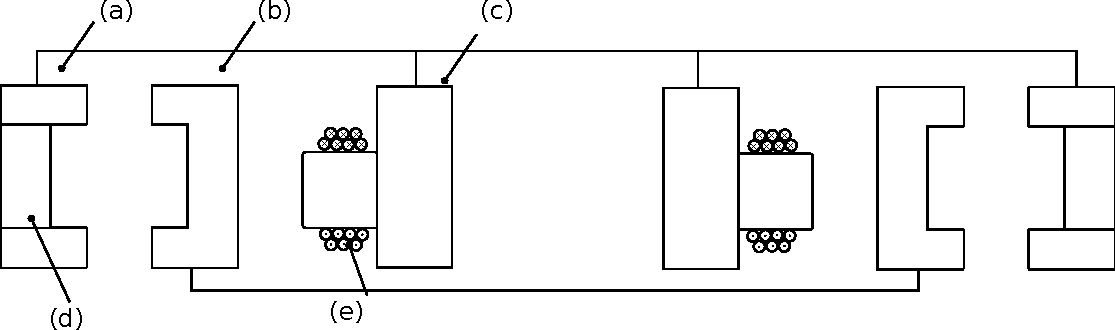
\includegraphics[width=1\linewidth]{Figs/mancais/mancal_corte2}
		\caption{Radial cut of the proposed magnetic bearing. (a) External stator; (b) Rotor; (c) Internal stator; (d) Permanent magnetics; (e) Coils}
		\label{fig:mancal:corte}
	\end{figure}
	
	\subsection{\uppercase{External Stator and Rotor}}
	
	A section of the magnetic circuit of the outer stator is illustrated in Figure \ref{fig:circuito:passivo}. The magnetic flux generated by the permanent magnet ($R_{ima}$) seeks the path of the minimal reluctance to close the magnetic circuit. This occurs by external stator irons ($\mathcal{R}_f$), then passing through the air gap ($\mathcal{R}_g$) and rotor ($\mathcal{R}_{fr}$). The permanent magnetic is a magnetic field source and is located between two irons. 
	The rotor undergoes attraction on all direction. At equilibrium (with a symmetrical air gap) the resultant force would tend to be null and remain in equilibrium at the operating point (critically stable). 
			
	\begin{figure}[ht]
		\subfigure[Magnetic circuit of the outer stator and rotor]{	
			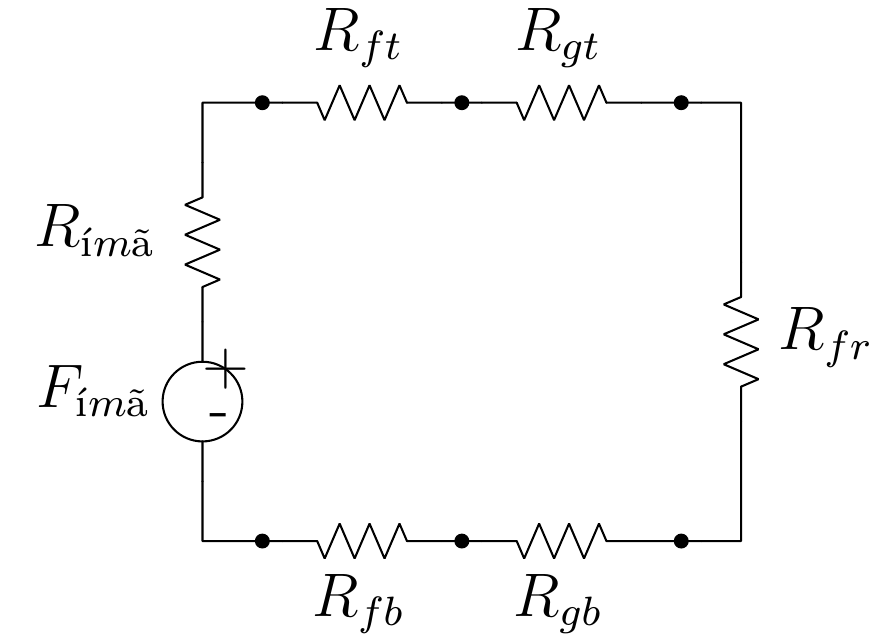
\includegraphics[width=0.4\linewidth]{Figs/circuito_passivo}
			\label{fig:circuito:passivo}
		}
		\hfill
		\subfigure[X and Y rotor displacement]{	
			\def\svgwidth{0.4\columnwidth}
			\includesvg{modelo_passivo_DxDy}
			\label{Fig:modelo:passivo:DxDz}
		}
		\caption{magnetic circuit of external stator and rotor }
	\end{figure}
	
	The magnetic field in the air gap (generated by the magnetics) can be decomposed into components $B_x$ and $B_z$ that are dependent on rotor displacement $\Delta_x$ and $\Delta_z$. The component z is responsible for stabilizing the passives degrees of freedom, the x component is a consequence of this topology causing the rotor instability on radial plane. Fig. \ref{Fig:modelo:passivo:DxDz} shows the magnetic flow on the external stator when displaced radially. 
			
	Magnetic attraction force $F$ can be calculated using the virtual work \citep{Chiba} it is a function of the magnetic field ($B(l)$) accumulated in the air gap and the area plus ($S(l)$) which $B$ is concentrated, as well as of the air permeability (permeability) ($\mu_0$). Eq. \eqref{eq:Force:virtualwork} is the described attraction force resulted from axial rotor displacement.
	
	\begin{equation}
			Fx = \frac{Bx(l)^2 \, S(l)}{2 \mu_0} ; \\
			Fz = \frac{Bz(l)^2 \, S(l)}{2 \mu_0}
			\label{eq:Force:virtualwork}
	\end{equation}
	
	
	Both magnetic field and air area are dependent of the air length ($l$), which makes the  attraction force non-linear.	Aiming the linearization of the attractive force, the outer stator is projected to work under magnetic saturation state making the quadratic portion of the equation constant ($B(l)^2 = cnt$) for small variations on gap length. Besides linearization, it is possible obtain with this technique a higher axial stiffness without a large increase in the radial one, which would require higher energy to stabilize actives degree of freedom. In order to make the tilt passive stable, the force generated in $F_z$ must be superior to $F_x $ for a predefined angle range (Fig. \ref{Fig:modelo:passivo:DxDz} otherwise the tilt would cause a non symmetric force on the rotor causing it to get unstable.
	
	By the development of an analytical model it was possible to choose initial construction parameters for this proposed topology and then an finite element model was created to develop and verify the topology. The aim of this step is to get a good axial rigidity ($F_z$) with a small  radial force ($F_x$). Fig. \ref{fig:forca:passivo:fx} shows the result of rotor when subjected to radial displacement, it is remarkable the linear force resulted from this topology, by the other side, we have a non linear attraction force for axial displacement (\ref{fig:forca:passivo:comsol:dy}).
	
	% Sergio acha que deveria explicar mais o pq é linear, mas já falei que a componente quadratica fica cnst para pequenas variações.
		
	\begin{figure}[ht]
		\subfigure[3D map of attraction force on the radial direction due to passive bearing system]{	
			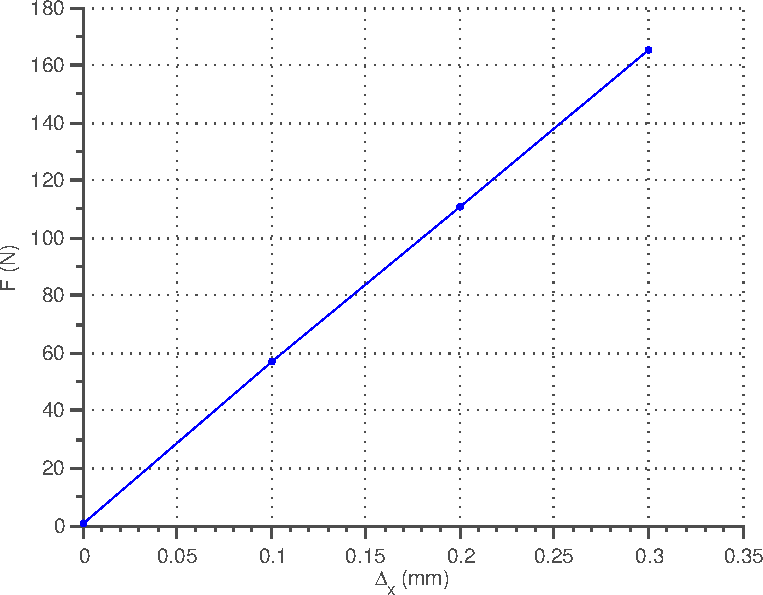
\includegraphics[width=0.5\linewidth]{./Figs/Simulacoes/Passivo/forca_passivo_comsol_fx}
			\label{fig:forca:passivo:fx}
		}
		\hfill
		\subfigure[X and Y rotor displacement]{	
			%{\textit{Magnetic Force (N) x Displacement Y (mm): Equilibrium point}}\\
			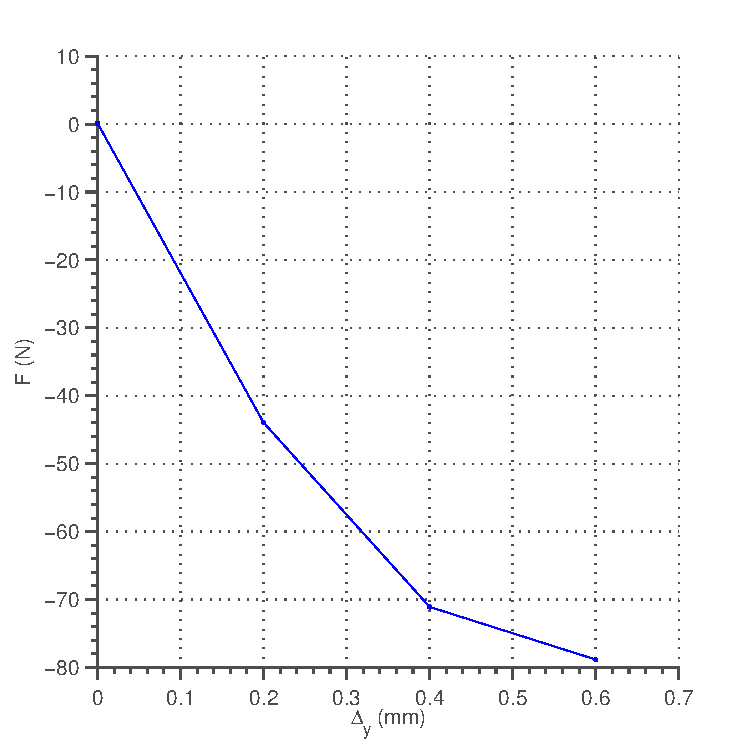
\includegraphics[width=0.45\linewidth]{./Figs/Simulacoes/Passivo/forca_passivo_comsol_dy}
			\label{fig:forca:passivo:comsol:dy}
		}
		\caption{Attraction force due to the passive circuit}
		\label{fig:forca:passivo}
	\end{figure}	
	
%	Is possible to write the attraction force on the radial axis as :
%	
%	\begin{equation}
%		F_p(x) = K_p x = 60k \, x
%	\end{equation}		
	
	\subsection{\uppercase{Inner stator and Rotor}}
	
	The inner stator contains eight magnetic poles evenly distributed at 45 degrees, connected by a internal circulation ring (component C of Fig. \ref{fig:mancal:corte}). The poles act as electromagnet generating attraction force to stabilize the rotor on the radial direction (x, y). Each trio of poles acts as a single actuator, forcing the flux to cycles by specifics poles maximizing the attraction force on the desired axis.
	
	Figure \ref{fig:modelo:mancal:estator:interno:fluxo} shows the internal stator with three poles acting as a single actuator: (A), (B), (C) and the respective magnetic flow generated by a current applied on the coils. Poles (A) and (C) work with inverse polarity of (B) forcing all magnetic flow through (B) and not by any other pole, thus maximizing the force of attraction $F_B$. The applied current on (A) and (C) is half of the current in the main pole (B) to prevent saturation.	Forces $F_A$ and $F_C$  have components in both directions x and y. For small changes on the operation point (nominal air length), the components in the y ($F_y$) direction is canceled because the same force vector is applied with opposite directions, in this example, $F_A$ and $F_B$. Leading to a single force in the x direction ($F_x$). Eq \ref{eq:ativo:F:resultante:x} is the resulted attraction forces on this situation.	
	
	\begin{equation}
		\vec{F}_x = \vec{F}_B + \cos(45) (\vec{F}_{A} + \vec{F}_{C}) \; ;\\
		\vec{F}_y =  \cos(45) (\vec{F}_{A} - \vec{F}_{C}) = 0 \label{eq:ativo:F:resultante:x}
	\end{equation}	
	

	
	\begin{figure}[ht]
		\centering
		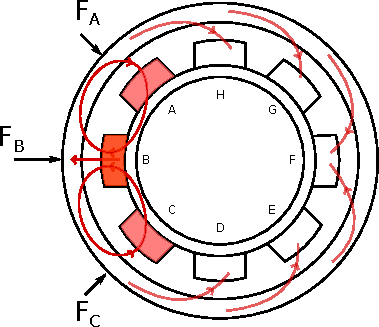
\includegraphics[width=0.6\linewidth]{./Figs/modelo_mancal_estator_interno_fluxo}
		\caption{Magnetic flux of active bearing system where A to H are the inner stator poles}
		\label{fig:modelo:mancal:estator:interno:fluxo}
	\end{figure}
	
	The initial geometric parameters of the internal stator were found by analyzing the power restriction. The maximum power for the system is 100W with a  supply voltage of 24V, resulting in a 4A max current. This electric current must be sufficient to generate an attraction force capable of compensate the force created by passive circuit under largest possible gap (Fig. \ref{fig:forca:passivo:fx}, $\Delta_x = 0.35$). From the analytic magnetic force model (Eq. \eqref{eq:ativo:F:resultante:x}) was possible to find a initial set of parameters (which include: areas, coil turns and air gap) able to generate a restorative force on the rotor with the imposed power restrictions. With a refined finite element model was possible to determine a better set of parameters by removing the unwanted saturated zones and maximizing the magnetic field on the gap by increasing the pole air area. Figure \ref{fig:forca:ativo} shows the achieved attraction force due the inner stator poles. This actuator has different gain depending on rotor position ($d_x$), larger the gap (negative dx) smaller the attraction force generated by the same current.
	
	\begin{figure}[ht]
	\centering
	\includegraphics[width=0.7\linewidth]{/Simulacoes/Ativo/mapa_forcas_ativo_comsol}
	\caption{Achieved attraction force on active circuit}
	\label{fig:forca:ativo}
	\end{figure}		
		
	\subsubsection{\uppercase{Inductance}} \label{subsec:at:indutancia}
	
	Inductance plays a crucial role in the performance of the actuator because its dynamic is correlated with the generation capacity (magnetic) of each pole and its current. Increasing the magnetic efficiency (in relation to the applied current) on poles results on a better attraction force, on the other hand,  generates a higher inductance that is worst in terms of dynamic response. For the present topology, the achieved inductance for each coil is $56 mH$ with an electrical resistance of $4 \Omega$. 
		
	\subsection{\uppercase{Resultant bearing}}
	
	The magnetic bearing has an external radius of 75.8 mm and max height of 18.0 mm. The nominal air length between the rotor and the external stator is 1.2 mm and 0.6 mm to the internal stator, the rotor mass is approximately 0,37 kg and axial stiffness is 60 kN/m. Fig. \ref{fig:prototipo} is an image of the constructed magnetic bearing prototype without the top stator iron.
	 
	\begin{figure}[ht]
	\centering
	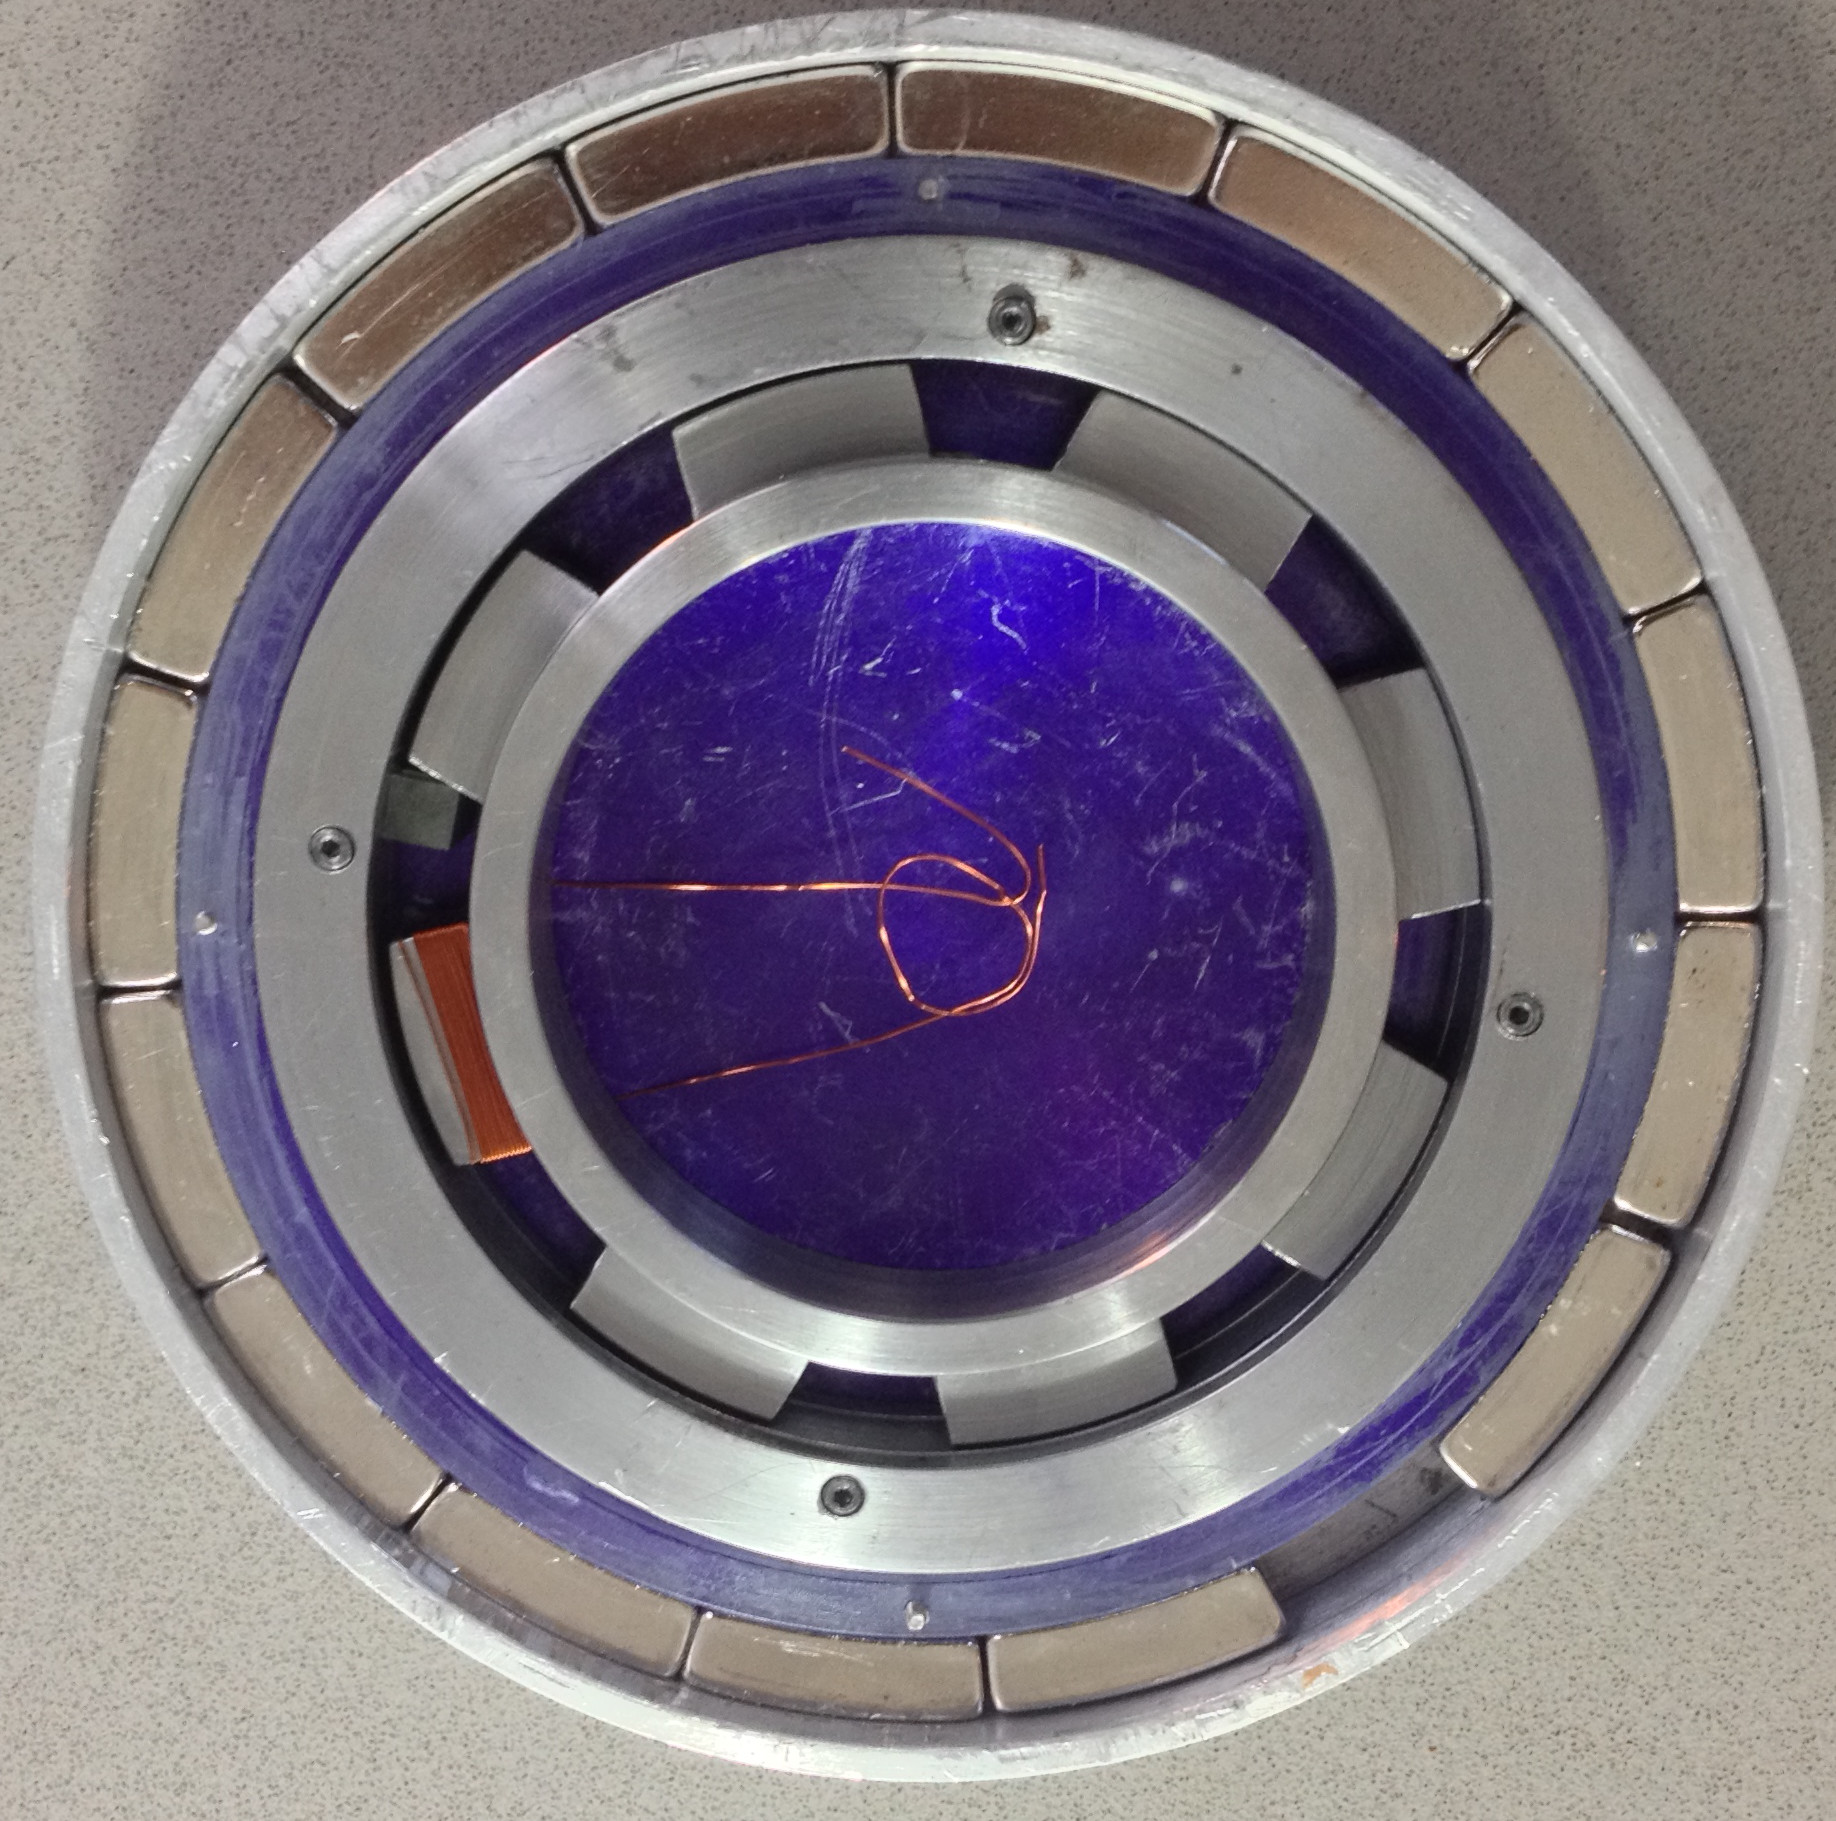
\includegraphics[width=0.4\linewidth]{/mancais/prototipo.jpg}
	\caption{First magnetic bearing prototype}
	\label{fig:prototipo}
	\end{figure}	
	
	\section{\uppercase{Dynamic Model}}

	The main rotor dynamics is basically influenced by its rotation speed ($\dot{\theta}$), inertia ($I$), mass ($m$) and air gap length ($l_g$) that can be  translated to rotor position : $dx,dy,dz$, composing all the kinetic energy (T). The potential energy (V) is due to axial translation (z), gravity (g) and by the passive bearing stiffness ($K_z$) shown in Fig. \ref{fig:forca:passivo:comsol:dy} : 
	
	\begin{align}
		T_{\theta, x, y, z} &= \frac{1}{2} I_z \, \dot{\theta}^2 + \frac{1}{2} \, m \, \left( \dot{x}^2 + \dot{y}^2 + \dot{z}^2 \right) \notag \\
		V_z &= m \, g \, z + \frac{1}{2} \, K_z \, z^2
	\end{align}	

	Two different forces act on the rotor: the  non-conservative forces ($Q^{nc}$) caused by the force applied by the actuators ($F_b$) that are depended on the rotor position and on the applied current ($i$); Conservative ($Q^{c}$) forces (which depend only on the position of the rotor) resulted from the passive attraction force ($K_p$). Both $F_b$ and $K_p$ are got from the calculated force by finite element model, respectively shown on Fig. \ref{fig:forca:ativo} and Fig. \ref{fig:forca:passivo:fx}.

	\begin{align}
		Q_y^{nc} &= F_{by}(dx,i)  \\
		Q_x^{nc} &= F_{bx}(dy,i)  \\
		Q^{c}_x  &= K_p \, dx \\
		Q^{c}_y  &= K_p \, dy 
	\end{align}
	
	Differential dynamic model can be obtained by applying the Lagrange formalism on previews equations, resulting on the following model:
			
	\begin{align}
		I \ddot{\theta} &= 0 \\
		m \ddot{x}		&= K_p \, dx  - F_{bx}(dx,i) \\
		m \ddot{y}		&= K_p \, dy  - F_{by}(dy,i)\\	
		m \ddot{z}  	&= K_z \, dz + m g 
	\end{align}
	
	Theses equations shows an uncoupled system (considering balanced). Both x and y directions must be active controlled by $F_b$ to overcome the attractive force ($K_p$) generated to stabilize the z direction. 
		
	Actuator dynamics is primarily caused by coil's electrical resistance (R) and inductance dependent on the operation point (L(x,y)). At the operation point, the resulted actuator has cut-off frequency of $11Hz$. The actuator dynamic ($G_a(S)$) is :
	
	\begin{align}
		G_a(s) = \frac{1}{L(dx,dy) \, s + R} 
	\end{align}
	
	Magnetic bearing radial dynamic model can be represented by the block diagram on Fig. \ref{fig:diagrama_blocos_modelo_linear}. A controller ($C(s)$) is needed to stabilities the system controlling the current on actuators ($i$), the controller is project to work as regulatory ($R=0$) since the bearing is project to work at  operation point ($dx=0, dy=0$).	Open loop transfer function used to project controller is derivate on Eq. \ref{eq:MA}.
	
	\begin{equation}
	dx = i_x \frac{K_b(dx,dy)}{[m s^2 - K_p (dx,dy)] \; [L(dx,dy) \, s + R] } 
	\label{eq:MA}
	\end{equation}
	
	\begin{figure}[!ht]
	\centering
	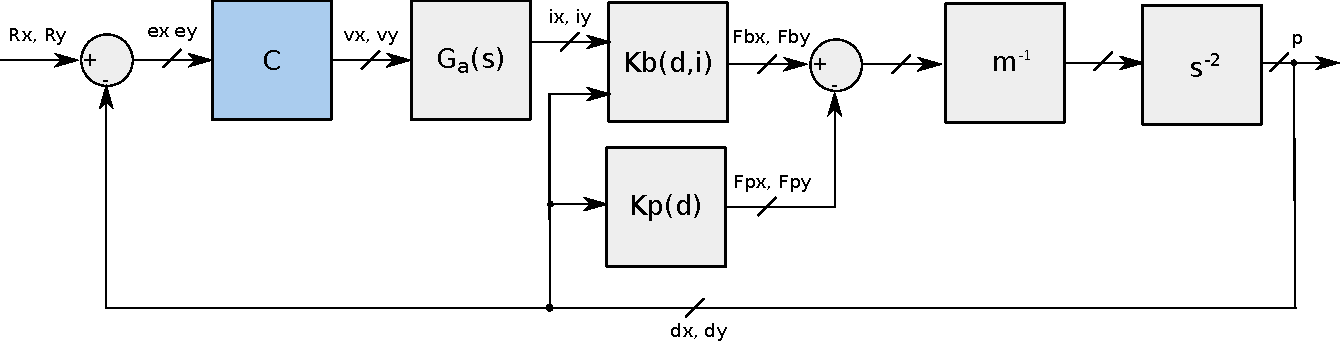
\includegraphics[width=1\linewidth]{Figs/Modelagem/diagrama_blocos_modelo_linear}
	\label{fig:diagrama_blocos_modelo_linear}
	\end{figure}	
	

	
	\section{\uppercase{CONTROLLER}}
	
	To overcome the non linearity on actuator gain ($Kb(d,i)$), a force control is designed instead of a current controller. The calculated force is applied to an estimator in order to calculate the current based on force and rotor position. Fig. \ref{fig:diagrama_controlador_estimador} is the proposed control scheme. Eq. \ref{eq:estimator:i} is the proposed current-force estimator, it is dependent on applied current ($I$), air gap length ($d$) and pole area  ($S_g$) obtained from a simplified electromagnetic model, Eq. \ref{eq:estimator:i} is the resulted current-force estimator.
		
	\begin{equation}
	I = \sqrt{\frac{2 \, F \, \mu_0}{S_g(d)}} \, \frac{\mu_0 \, S_g(d)^2}{n}
	\label{eq:estimator:i}
	\end{equation}
	
	\begin{figure}[ht]
	\centering
	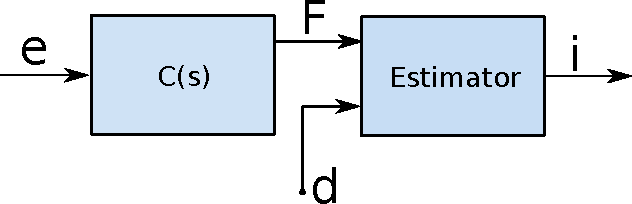
\includegraphics[width=0.3\linewidth]{Figs/Modelagem/controlador_estimador}
	\caption{Proposed controller scheme with current estimator}
	\label{fig:diagrama_controlador_estimador}
	\end{figure}
		
	A SISO loop-shaping controller ($H_{\infty}$) \citep{skogestad2007multivariable} was designed to stabilize the rotor at it operational point  in order to have a good margin between the nominal (linearized) plant and the real one (non linear). The controller model the system frequency response to a first order low pass filter with cut-off-frequency of $100$ rad/s and a zero DC gain.
	
	Fig. \ref{fig:controlled} is a simulation of the controlled system. This simulation the controller is initially disabled and initial condition takes the rotor from the equilibrium position to the shock with external stator (dy = 0.35 mm and dx = 0.18 mm). The controller is activated at 0.1 second and takes 0.3 seconds to recover the rotor from the worst case to its nominal position with 0.5 A of current peak. A disturbance of 0.01 mm is applied to dx position at 0.5 seconds. 
	
	\begin{figure}[ht]
	\centering
	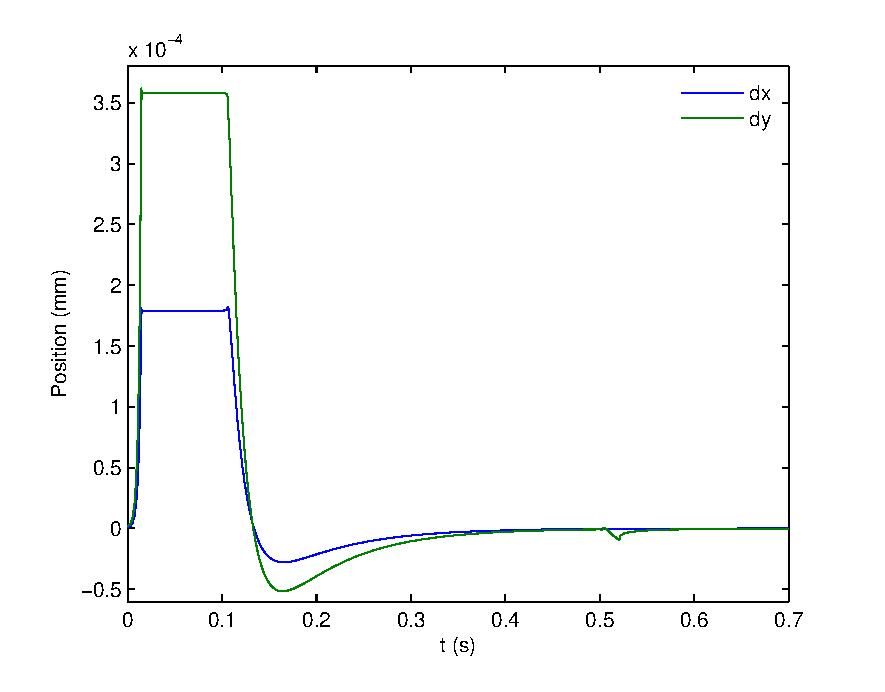
\includegraphics[width=0.7\linewidth]{./Figs/Modelagem/controlled_time.eps}
	\caption{Simulated controlled plant time response}
	\label{fig:controlled}
	\end{figure}	
	
	\section{CONCLUSION AND FUTURE WORKS}
	
	In this paper a new topology of magnetic bearing system aiming the application on satellite reaction wheel is develop, suggested bearing respects restrictions dimensions, mass and power consumption restrictions. A control with low position oscillation and good performance against perturbation is proposed.	Future work are in line to have a more complete electromagnetic model aiming optimizations on the proposed topology. A first functional prototype with position sensors and drive electronics is under construction and will help to push the development of others subsystems of the reaction wheel.
		
	\section{ACKNOWLEDGEMENTS}
	
	 Thanks to Instituto Mau\'{a} de Tecnologia and Dr. Leonardo Pinheiro that made this project possible.
	
	\section{REFERENCES} 
	
	\bibliographystyle{cobem2015}
	\renewcommand{\refname}{}
	\bibliography{./bibfile}
	
	\section{RESPONSIBILITY NOTICE}
	
	The authors are the only responsible for the printed material included in this paper.
	
\end{document}
